\documentclass[10pt]{article}

\usepackage[utf8]{inputenc}
\usepackage[T1]{fontenc}
\usepackage[francais]{babel}
\usepackage{setspace}
\usepackage{fancyhdr}
\usepackage{verbatim}
\usepackage{listings}
\usepackage{graphicx}
\usepackage[top=2cm, left=2cm, right=2cm]{geometry}

\lstset{columns=flexible,
	basicstyle=\ttfamily\footnotesize,
	frame=simple,
	showstringspaces=false}


\pagestyle{fancyplain}

\lhead{\footnotesize\sf Projet BD}
\rhead{\footnotesize\sf Equipe \bsc{Teide} 1}


\title{Compte-rendu du projet Base de Données\\ \emph{Gestion d'un centre de vacances}}
\author{\bsc{Garcia Maxime - Ghorreshi Omid}\\ \bsc{Havet Corentin - Portelenelle Brice} \\(\bsc{Teide} $1$ ; \bsc{TD} G1)}
\date{Mai 2015}


\begin{document}
\maketitle

\tableofcontents

\newpage
\section{Analyse du problème}

L'analyse du texte proposé par l'énoncé nous a amené aux dépendances fonctionnelles et contraintes suivantes.\\

\begin{small}
\begin{tabular}{|c|}

\hline
\\Dépendances fonctionnelles\\ \\
\hline

\\CodeCentre -> NomCentre, AdrPoste\\

NumeroResp -> CodeCentre, NomResp, PrenomResp, NaissanceResp, TelResp, MailResp, AdrPoste\\

AdrPoste -> NumAdr, RueAdr, CodeAdr, VilleAdr\\

CodeAct -> NomAct, CategorieAct, DescAct, NbMinStagiairesGroupe, NbMaxStagiairesGroupe, TypeMat\\

CodeMoniteur -> CodeCentre, NomMoniteur, PrenomMoniteur, NaissanceMoniteur, TelMoniteur, MailMoniteur, AdrPoste\\

CodeStagiaire -> NomStagiaire, PrenomStagiaire, NaissanceStagiaire, TelStagiaire, MailStagiaire, AdrPoste\\

NumSeance, CodeGroupe -> DateSeance, HeureDebut, Duree\\

NumMateriel, CodeCentre -> TypeMat, MarqueMat, ModeleMat, NiveauMat, QuantiteMat\\

CodeMoniteur, CodeAct -> NbMaxStagiairesMoniteur\\ \\

\hline
\\Contraintes de valeurs\\ \\
\hline

\\NbMinStagiairesGroupe > 0 \\

NbMaxStagiairesGroupe > 0\\

NbMaxStagiairesMoniteur > 0\\

CategorieAct IN ('nautique', 'montagne', 'air')\\

DateDebGroupe < DateSeance < DateFinGroupe\\

DateSeance à l'heure HeureDebut + Durée < DateFinGroupe à 24h00\\

Durée > 0\\

NiveauGroupe IN ('debutant, 'confirme' , 'expert')\\

NiveauMat IN ('debutant', 'confirme', 'expert'), QuantiteMat >= 0\\

NbMaxStagiairesMoniteur > 0\\

Activite(TypeMat) peut être NULL\\ \\

\hline
\\Contraintes de multiplicité\\ \\
\hline

\\Un moniteur peut etre un responsable\\

Chaque activité nécessite l'utilisation d'un ou plusieurs matériels : QuantitéMat = 0, l'activité ne peut plus être 
effectuée\\

Les moniteurs peuvent encadrer une ou plusieurs activités dont ils ont l'habilitation. Il peut être responsable.\\

Un stagiaire peut s'inscrire dans plusieurs centres, mais à des périodes disjointes\\

Un groupe est composé de stagiaires qui suivent tous la même activité pendant la même période\\

Chaque séance est encadrée par un ou plusieurs moniteurs selon les normes de sécurité de l'activité\\

Un stagiaire peut appartenir à plusieurs groupes ou meme à aucun groupe.\\ \\

\hline
\\Autres contraintes\\ \\
\hline

\\Les stagiaires s’inscrivent dans un centre pour une période définie par une date de début et une date de fin.\\

Un groupe correspond à un niveau de pratique de l’activité (débutant, confirmé ou expert)\\

Il faut savoir quel(s) matériel(s) sont utilisés par chaque séance des groupes et en quelle quantité.\\

La quantité de matériel de la séance varie selon la date, l'heure de début, l'heure de fin de la séance\\ \\

\hline

\end{tabular}
\end{small}

\section{Conception Entités/Associations}

A partir de ces différentes dépendances fonctionnelles et certaines contraintes, nous avons pu réaliser le schéma entités/associations
ci-dessous.

\begin{figure}[h!]
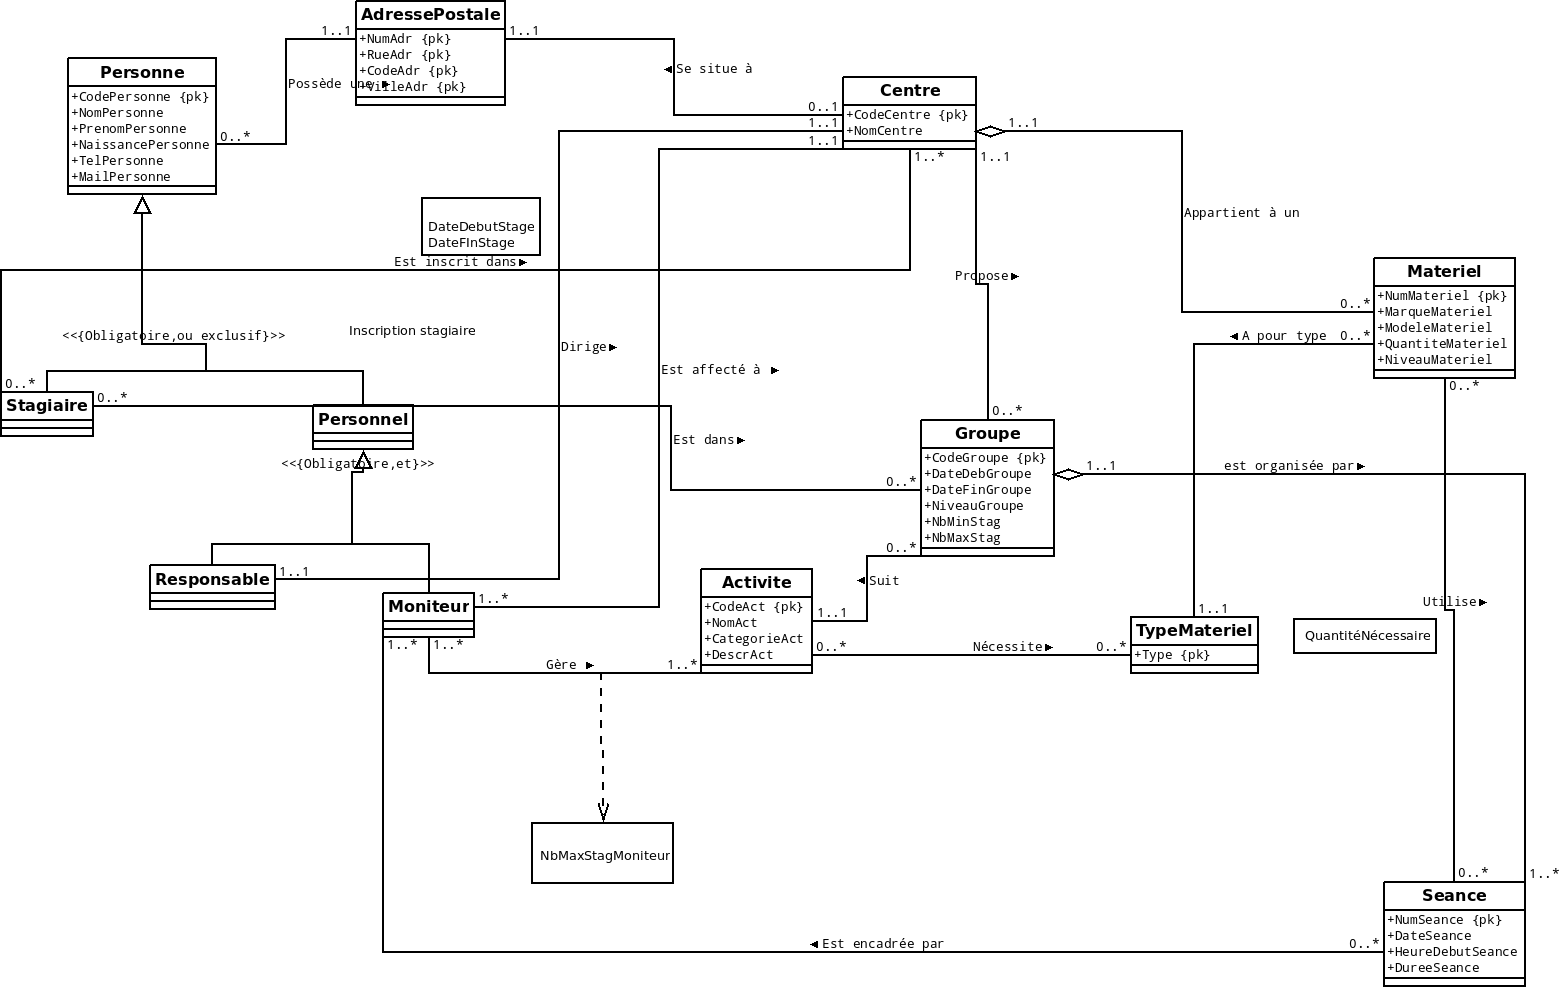
\includegraphics[scale=0.3]{DiaVLV.png}
\caption{Modèle Entités/Associations}
\end{figure}

\section{Passage au schéma relationnel}

Afin de passer du modèle entités/associations au schéma relationnel, on a appliqué linéairement les consignes de la feuille du cours,
\emph{i.e.} on a traité tout d'abord les associations reliant une entité faible, puis les associations de cardinalité ($1..1$) non encore
traitées, puis celles avec cardinalité ($0..1$) non encore traitées, puis celles avec (x$..*$) et enfin les associations ternaires ou plus.

Nous obtenons le schéma relationnel suivant, où apparaissent les contraintes que l'on a pu y insérer et où l'on a séparé les différents
types d'entités.

\subsection{Entités simples}


\begin{small}

\textbf{Centre (\underline{CodeCentre}, NomCentre, NumAdr, RueAdr, CodeAdr, VilleAdr)}

    \hspace{1cm}NumAdr, RueAdr, CodeAdr, VilleAdr non nuls et référencent  AdressePostale
    
    \hspace{1cm}CodePersonne référence Responsable\\

\textbf{Groupe (\underline{CodeGroupe}, CodeCentre, CodeAct, DateDebGroupe, DateFinGroupe, NbMinStagGroupe, NbMaxStagGroupe, NomNiveau)}

    \hspace{1cm}Vérifier qu’un Groupe organise au moins une Seance
    
    \hspace{1cm}NomNiveau non nul référence Niveau
    
    \hspace{1cm}CodeCentre référence Centre
    
    \hspace{1cm}CodeAct référence Activité\\

\textbf{EstDansGroupe (\underline{CodePersonne}, \underline{CodeGroupe})}

    \hspace{1cm}CodePersonne référence Stagiaire
    
    \hspace{1cm}Un Groupe contient entre nbMin et nbMax Stagiaire\\

\textbf{Personne (\underline{CodePersonne},NomPersonne, PrenomPersonne, NaissancePersonne, TelPersonne, MailPersonne, NumAdr, RueAdr, 
CodeAdr,VilleAdr)}

    \hspace{1cm}NumAdr, RueAdr, CodeAdr, VilleAdr non nuls et référencent  AdressePostale\\

\textbf{AdressePostale (\underline{NumAdr}, \underline{RueAdr}, \underline{CodeAdr}, \underline{VilleAdr})}\\

\textbf{Activite (\textbf{CodeAct}, NomAct, CategorieAct, DescrAct)}

    \hspace{1cm}Vérifier qu’une Activite est gérée par au moins un Moniteur
    
    \hspace{1cm}Vérifier qu’une Activite nécessite au moins un Materiel\\   

\textbf{Gère (\underline{CodePersonne}, \underline{CodeAct}, NbMaxStagMoniteur)}

\hspace{1cm}Vérifier que CodePersonne est un Moniteur\\

\textbf{Nécessite (\underline{CodeAct}, \underline{Type})}

    \hspace{1cm}CodeAct référence Activité
    
    \hspace{1cm}Type référence TypeMateriel\\

\textbf{Utilise(\underline{CodeGroupe},\underline{NumSeance},\underline{CodeCentre},\underline{NumMateriel}, QuantiteNecessaire)}
    
    \hspace{1cm}Vérifier que Groupe(CodeGroupe).CodeCentre = CodeCentre\\

\textbf{TypeMateriel(Type)}\\

\textbf{EstEncadreePar (\underline{CodePersonne},\underline{CodeGroupe},\underline{NumSeance})}

    \hspace{1cm}CodePersonne référence Moniteur
    
    \hspace{1cm}Personne(CodePersonne).CodeCentre = Groupe(CodeGroupe).CodeCentre
    
    \hspace{1cm}Gere(CodePersonne,Groupe(CodeGroupe).CodeAct) existe
    
    \hspace{1cm}Gere(CodePersonne,Groupe(CodeGroupe).CodeAct).NbMaxStagMoniteur >= nb de personnes dans le groupe\\

\textbf{EstInscritDansCentre (\underline{CodePersonne}, \underline{CodeCentre})}
    
    \hspace{1cm}CodePersonne référence Stagiaire
    
    \hspace{1cm}Vérifier qu’un Stagiaire est inscrit dans au moins un Centre\\
    
\end{small}

\subsection{Entités faibles}

\begin{small}

 \textbf{Materiel (\underline{CodeCentre}, \underline{NumMateriel}, Type, MarqueMateriel, ModeleMateriel, QuantiteMateriel, NomNiveau)}
 
    \hspace{1cm}CodeCentre référence Centre 
    
\hspace{1cm}NomNiveau non nul référence Niveau

\hspace{1cm}Type non nul référence TypeMateriel\\

\textbf{Séance (\underline{CodeGroupe}, \underline{NumSeance}, DateSeance, HeureDebutSeance, DureeSeance)}

    \hspace{1cm}CodeGroupe référence Groupe\\
    
\end{small}

\subsection{Sous-types d'entités}

\begin{small}

 \textbf{Stagiaire (\underline{CodePersonne}) }
 
    \hspace{1cm}CodePersonne référence Personne\\

\textbf{Responsable (\underline{CodePersonne}, CodeCentre)}

    \hspace{1cm}CodePersonne référence Personne
    
    \hspace{1cm}CodeCentre référence Centre\\

\textbf{Moniteur (\underline{CodePersonne}, CodeCentre)}

    \hspace{1cm}CodePersonne référence Personne
    
    \hspace{1cm}CodeCentre référence Centre
    
    \hspace{1cm}Vérifier qu’un Centre emploi au moins un Moniteur
    
    \hspace{1cm}Vérifier qu’un Moniteur encadre au moins une Activite\\
    
\end{small}


\section{Analyse des fonctionnalités et implémentations en SQL}

\subsection{Enregistrement d'un stagiaire à un centre et à une activité}

\subsection{Création et suppression d'un groupe}

\subsection{Planification d'une séance pour un groupe}

\subsection{Visualisation des séances planifiées}

C'est une requête SQL qui ne nécessite pas d'interaction de l'utilisateur ou de vérification à l'aide de \emph{JDBC}.

On affiche la table \textbf{Seance}. Cette table est affichée dans l'ordre des \textbf{CodeGroupe} et des \textbf{NumSeance}.

On a donc trouvé la requête SQL :
\begin{small}
\begin{verbatim}
SELECT *
FROM seance;
\end{verbatim}
\end{small}

\subsection{Gestion du matériel (inventaire, ajout, suppression)}

\subsubsection{Inventaire du matériel}

C'est une requête SQL qui ne nécessite pas d'interaction de l'utilisateur ou de vérification à l'aide de \emph{JDBC}.

On affiche la table \textbf{Materiel}. Cette table est affichée dans l'ordre des \textbf{CodeCentre} et des \textbf{NumMateriel}.

On a donc trouvé la requête SQL :
\begin{small}
\begin{verbatim}
SELECT *
FROM materiel;
\end{verbatim}
\end{small}

\subsubsection{Ajout du matériel dans un centre}

On affiche la liste des \textbf{CodeCentre}. On demande alors le centre dans lequel on veut ajouter du matériel. Ensuite,
on affiche la liste des matériels du centre. On demande alors quel matériel on veut ajouter et en quelle quantité. On renvoie une exception si l'utilisateur donne une réponse incohérente.

On utilise les requêtes SQL suivantes :

\begin{small}
\begin{verbatim}
select CodeCentre
from centre;

-- Dans quel centre voulez-vous ajouter du materiel ? Reponse : codecentre = i
select *
from materiel 
where codecentre = i;

-- Quel matériel voulez-vous ajouter ? Reponse : nummateriel = j
-- Quel quantite voulez-vous ajouter ? Reponse : k
update materiel
	set QuantiteMateriel = QuantiteMateriel + k
	where codecentre = i AND nummateriel = j;
\end{verbatim}
\end{small}

\subsection{Pour chaque activité, classement des centres en fonction du nombre d'inscrits}

C'est une requête SQL qui ne nécessite pas d'interaction de l'utilisateur ou de vérification à l'aide de \emph{JDBC}. 

On a fait un GROUP BY sur les noms d'activités et des centres pour le calcul du nombre d'inscrits, et on a ordonné les tuples trouvés 
selon les noms d'activités et le nombre d'inscrits, comme demandé par l'énoncé.

On a donc trouvé cette requête SQL :

\begin{small}
\begin{verbatim}
SELECT DISTINCT a.NomAct, c.NomCentre as Centre, count(*) as Nb_Inscrits
FROM Activite a, EstDansGroupe edg, Centre c, Groupe g
WHERE edg.CodeGroupe = g.CodeGroupe AND g.CodeAct = a.CodeAct AND g.CodeCentre = c.CodeCentre
GROUP BY a.NomAct, c.NomCentre
ORDER BY a.NomAct, Nb_Inscrits;
\end{verbatim}
\end{small}

\subsection{Classement des villes par nombre de stagiaires inscrits}

C'est une requête SQL qui ne nécessite pas d'interaction de l'utilisateur ou de vérification à l'aide de \emph{JDBC}. 

On a tout d'abord fait un groupement par ville où un centre est présent, en calculant le nombre d'inscrits par ville.
Puis, les villes où aucun centre n'est présent ne s'affichant, on a fait une union avec les tuples précédents afin d'afficher $0$ 
pour le nombre d'inscrits dans les villes restantes.

On a donc trouvé cette requête SQL :

\begin{small}
\begin{verbatim}
SELECT DISTINCT ap.VilleAdr as Ville, count(i.CodePersonne) as Nb_Inscrits
FROM Centre c, EstInscritDansCentre i, Adresse_Postale ap
WHERE ap.VilleAdr = c.VilleAdr AND ap.NumAdr = c.NumAdr AND ap.RueAdr = c.RueAdr AND ap.CodeAdr = c.CodeAdr 
      AND i.CodeCentre = c.CodeCentre
GROUP BY ap.VilleAdr
UNION
SELECT DISTINCT ap.VilleAdr as Ville, 0
FROM Adresse_Postale ap, Centre c
WHERE ap.VilleAdr NOT IN (	SELECT c.VilleAdr
      		      	 	FROM Centre c, EstInscritDansCentre i
				WHERE c.CodeCentre = i.CodeCentre	)
ORDER BY Nb_Inscrits;
\end{verbatim}
\end{small}

\section{Bilan du projet}

\subsection{Organisation}

Tous les membres de l'équipe se retrouvaient à chaque séance encadrée, les mardi matins et vendredi après-midi, afin de travailler 
ensemble et de minimiser le travail à faire en dehors des séances.\\

Nous avancions bien, en posant des questions à l'encadrant lorsque nous ne savions pas comment faire, surtout en le considérant comme
client, car le texte était obscur sur certains points. 
Nous travaillions sur \emph{Google Drive} afin de voir les changements effectués, et d'en faire, en temps réel. Pour le début, cela était
bien pratique car nous rajoutions chacun ce que l'on avait compris du texte. Si un n'était pas d'accord, il le voyait immédiatement et
on corrigeait assez vite après discussion. \\

Ensuite nous nous sommes séparés en deux binômes, un travaillant sur le modèle entités/associations, et l'autre sur le schéma relationnel.
Il faut normalement attendre la fin du premier pour faire le second, c'est pourquoi au départ le deuxième binôme aidait le premier, mais
une fois que le schéma entités/associations était assez conséquent et relu, le deuxième binôme a attaqué le passage au relationnel.
Bien sûr il a parfois fallu modifier le diagramme, et cela impliquait de petites modifications dans le schéma relationnel. Mais faire
le schéma relationnel à peu près en parallèle permettait de se poser des questions sur le diagramme, et donc de clarifier certains
points.\\

Ensuite, un binôme s'était occupé des créations de tables et des insertions de tuples afin de tester celles-ci, et l'autre binôme 
s'occupait des requêtes SQL à faire. Enfin, vers la fin du projet, tout le monde faisait ce qu'il restait à faire, avec chaque membre
de l'équipe ayant apporté sa contribution au code Java et aux insertions de tuples pour étoffer la base.

\subsection{Points difficiles}

Les difficultés rencontrés ont surtout été certains points de compréhension lors de la première analyse du texte. Ainsi poser des questions
à l'encadrant en le considérant comme le client était indispensable pour que nous puissions avancer. \\

Ensuite il s'agissait de bien passer au modèle entités/associations, ce qui nous amenait à nous poser des questions également, notamment
en ce qui concerne les cardinalités ou certaines entités à mettre au final en attribut ou non. \\

Pour le reste, il s'agit surtout des vérifications Java qui nous ont posé quelques problèmes. En effet, il fallait savoir lesquelles
faire, et comment le faire avec \emph{JDBC}. \\

En somme, la majorité des difficultés que nous avons rencontrées étaient dues à des points peu clairs de l'énoncé de départ, ce qui fait
que nous savions parfois pas que faire comme vérifications, qu'est-ce qui était autorisé ou non.

\subsection{Impressions}

Nous trouvons ce projet très intéressant pour la formation de l'ingénieur Ensimag, car il permet, comme le projet GL mais avec un
rythme moins soutenu, de nous plonger dans une documentation parfois peu claire, et d'en tirer un programme informatique répondant
à des spécifications, que nous devions parfois demander au client de clarifier. En ce sens ce projet dépeint correctement ce qui nous
attendra plus tard dans notre vie professionnelle, lors des échanges avec les clients, et cela nous a donc apporté un bon aperçu
du cheminement à mener en plus des connaissances en base de données que nous avons pu mettre en \oe{}uvre et consolider.

\end{document}
